% !TEX encoding = UTF-8 Unicode
% 予備審査レジュメ 2 ページ版(予備審査会で使う。4 ページ版は resume.tex)(特研1審査会のレジュメ 2025年度 を元にしたテンプレート)
% 図をページ幅で入れるため multicols ではなく twocolumn にした(11/22)
% ヘッダーは先輩(2025年度 7307)の「創造工学専攻 情報工学コース / 年度 特別研究 2 審査会」に合わせた
% ビルド:thesis/resume/ で latexmk resume.tex → build/resume.pdf
\documentclass[10pt,uplatex,dvipdfmx,twocolumn]{jsarticle}

% 描画・色関連
\usepackage[dvipdfmx]{graphicx}
\usepackage[dvipdfmx]{xcolor}
\usepackage{here}

% レイアウト調整関連
\usepackage{geometry}
\usepackage{setspace}
\usepackage{fancyhdr}
\usepackage{float}

% 数式関連
\usepackage{amsmath}
\usepackage{amssymb}
\usepackage{mathtools}
\usepackage{bm}

% 表・リスト関連
\usepackage{booktabs}
\usepackage{enumerate}

% テキスト装飾関連
\usepackage{url}

% キャプション関連
\usepackage{caption}
\usepackage{subcaption}

\graphicspath{{figures/}{../figures/}{../../experiments/}}
\geometry{a4paper, left=20mm,right=20mm,top=20mm,bottom=20mm}

\definecolor{tmcitblue}{cmyk}{0.86,0.91,0,0.04}
\pagestyle{fancy}
\fancyhf{}
\lhead{\color{tmcitblue}\footnotesize 東京都立産業技術高等専門学校}
\rhead{\color{tmcitblue}\footnotesize 専攻科 情報工学コース\\2026 年度特別研究Ⅱ予備審査会}
\lfoot{\color{tmcitblue}\footnotesize Tokyo Metropolitan College of Industrial Technology}
\cfoot{\thepage}
\renewcommand{\headrulewidth}{0.0pt}
\setlength{\headheight}{20.2781pt}
% ページ幅の図(figure*)をページの上に2つまで置けるように
\setcounter{dbltopnumber}{3}
\renewcommand{\dbltopfraction}{0.85}
\renewcommand{\dblfloatpagefraction}{0.85}
\renewcommand{\textfraction}{0.1}

% 2 ページに収めるため、節と図の前後の空きを詰める
\setlength{\textfloatsep}{8pt plus 2pt minus 2pt}
\setlength{\dbltextfloatsep}{8pt plus 2pt minus 2pt}
\captionsetup{skip=4pt}
\makeatletter
\renewcommand{\section}{\@startsection{section}{1}{\z@}{0.6\Cvs \@plus.3\Cdp}{0.3\Cvs}{\normalfont\large\headfont\raggedright}}
\renewcommand{\subsection}{\@startsection{subsection}{2}{\z@}{0.3\Cvs \@plus.2\Cdp}{0.1\Cvs}{\normalfont\normalsize\headfont}}
\makeatother

\begin{document}
\setstretch{1.00}
\twocolumn[{%
\centering
\Large{エッジマイクロクラスタにおける空間熱干渉を考慮した熱抑制手法の研究}\\
\vspace{6pt}
\large{7303 鈴木黎映}\\
\large{指導教員 知念賢一教授}
\vspace{10pt}
}]

\section{はじめに}
データセンタでは冷却設備の電力が全体の大きな割合を占め~\cite{dayarathna}、サーバの排熱が別のサーバの吸気側に回り込む熱の再循環が冷却の効率を下げる~\cite{moore,tang}。空調のない棚や箱に置かれるエッジのマイクロクラスタ~\cite{iridis}にも同じ問題があり、Raspberry Pi 4B(以下、Raspi)は CPU 温度が約 80\,℃ を超えるとクロックを下げ(スロットリング。公式の上限は 85\,℃ だが、実測では 80\,℃ から下がり始めた)、処理が遅くなる。ファンを常に回せば温度は下がるが、ファンの寿命は稼働時間で表されるため~\cite{kim}回し続けるほど寿命に近づき、騒音にもなる。

本研究では、スロットリングを避けつつファンの稼働をできるだけ減らすことを目指す。先行発表~\cite{ipsj}では、隣のノードの排熱で温度が上がる空間熱干渉を状態として推定するカルマンフィルタを提案した。しかし、予測に未来の実測値を用いていた、同定と評価に同じデータを用いていた、などの課題があった。本研究ではこれらを直し、30 秒先の温度とその不確かさを予測して、予測が安全閾値を超えるときだけファンを回す制御を実機で評価する。あわせて、空間熱干渉が実際にどの程度生じるかと、温度だけを見るしきい値方式と比べて、予測がどのような条件で有効になるかを明らかにする。


\section{関連研究}
Zanini ら~\cite{zanini}は、熱 RC モデルによるモデル予測制御でマルチコアの温度を管理した。坂本ら~\cite{sakamoto}は、予測に持たせるマージンを変動の大きさに応じて動的に変える方法を提案した。Coskun ら~\cite{coskun}や Yeo ら~\cite{yeo}は、温度を予測して先回りする熱管理が、上限に達してから処理を抑える反応的な方法より良いことを示したが、比べた反応的な方法は性能を下げる操作であった。データセンタでは、空調の給気温度のモデル予測制御~\cite{ogura}や、ラックの吸気温度の 30 分先の予測~\cite{sasakura}が研究されている。本研究は、性能を下げないノードごとのファンを操作し、予測を用いる方式と温度だけを見る方式を同じ冷却手段で実機で比べ、予測が有効になる条件を明らかにする点が異なる。

\section{提案手法}
5 秒ごとに温度・CPU 使用率 $u_t$・ファンの状態 $f_t$(0/1)を観測する。温度を室温からの上昇分 $\theta = T - T_{\mathrm{amb}}$ で表し、熱 RC モデルを離散化した次のモデルを用いる。
\begin{gather}
  \theta_{t+1} = a\,\theta_t + b\,u_t + c\,H_t + e\,f_t + d \\
  H_{t+1} = \rho\,H_t + (1-\rho)\,z_t
\end{gather}
$H_t$ は隣接ノードからの外部熱影響、$z_t$ は隣接ノードの温度の普段からの変化分である。$a$ は熱の残り方、$d$ は待機時の発熱を表し、$b > 0$(負荷による加熱)、$e < 0$(ファンによる冷却)、$c \ge 0$(隣の熱で冷えることはない)とする。状態 $[\theta_t, H_t]^\top$ をカルマンフィルタで推定し(隣の温度が急に変わると $H$ のプロセスノイズを大きくする)、今の負荷が続きファンは OFF のままと仮定して、30 秒先の温度と標準偏差 $\sigma$ を予測する。OFF と仮定するのは、「回さなくても安全か」を判断するためである。30 秒は、ファンが効くまでの時間(5 秒以内)より長く、温度の時定数(約 1〜2 分)より短い長さとして決めた。
\begin{equation}
  M_t = \alpha\,\sigma_t + \delta,\qquad T_{\mathrm{safe}} = T_{\mathrm{limit}} - M_t
\end{equation}
$\alpha = 2$、$\delta = 0.5$\,℃(温度センサの刻み)、$T_{\mathrm{limit}} = 80$\,℃ とした。誤差が正規分布に従えば、予測 $+ 2\sigma$ を実測が超える確率は約 2.3\% である。予測温度が $T_{\mathrm{safe}}$ を超えたらファンを ON にする(最小 ON 時間 30 秒、OFF は 1\,℃ のヒステリシス)。

\section{実験}
\begin{figure}[tb]
  \centering
  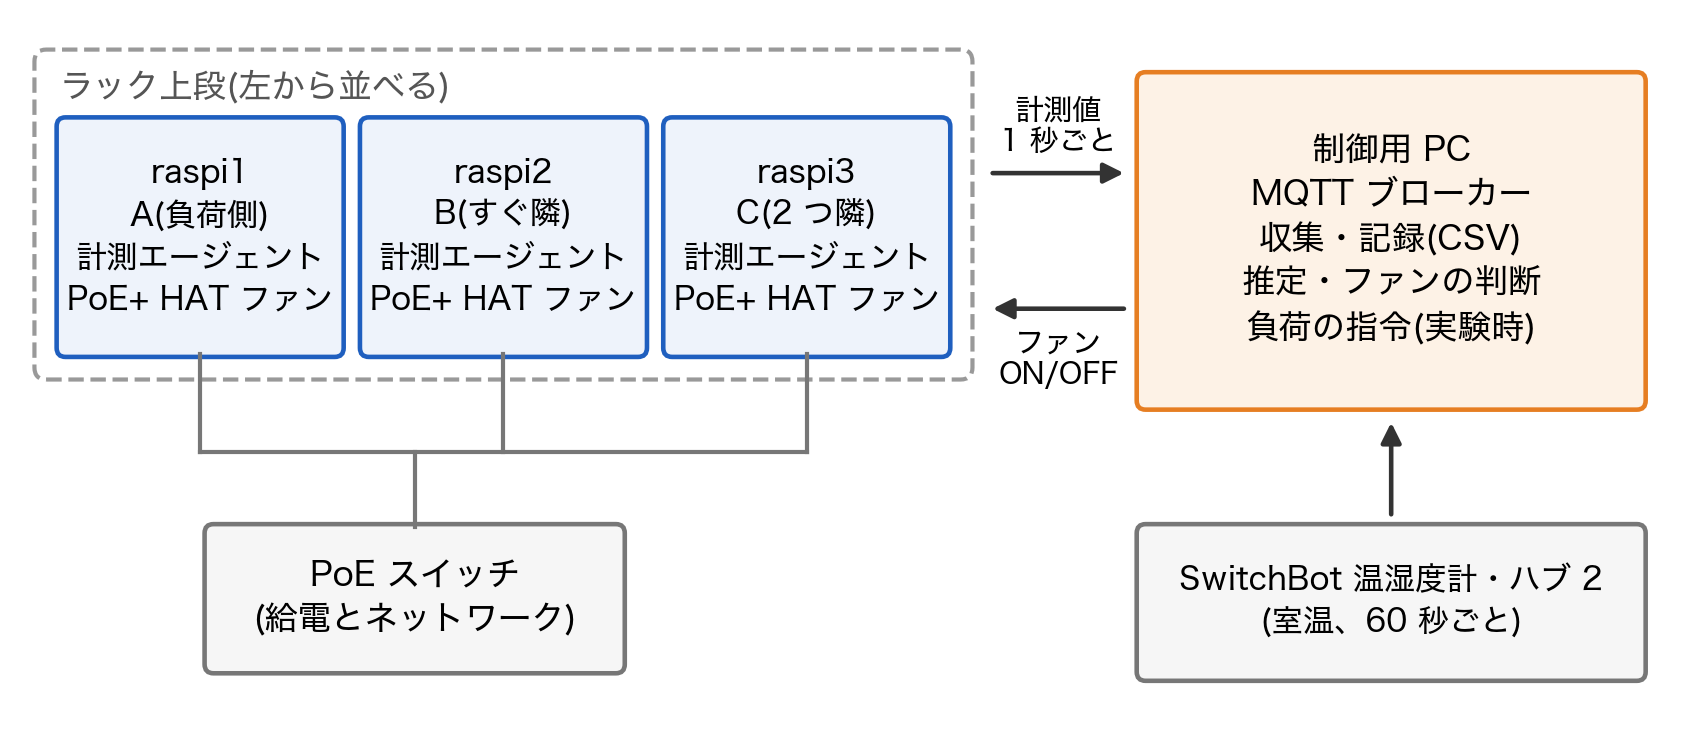
\includegraphics[width=\columnwidth]{fig_system.png}
  \caption{実験の構成。3台は 19 インチラックの上段に左から並べ、PoE スイッチから給電した}
  \label{fig:system}
\end{figure}
Raspi 3台(A、B、C)を 19 インチラックの上段に左から並べ(B は A のすぐ隣、C は2つ離れた位置)、PoE+ HAT(給電用の拡張基板)のファンを制御用 PC から ON/OFF した(図~\ref{fig:system})。1 秒ごとに温度・CPU 使用率・クロック・ファンの状態などを MQTT で集め、室温も記録した。負荷は \texttt{stress-ng} で与えた。

モデルのパラメータの同定と予測の評価には、3台の負荷(0〜4 コア)とファンの ON/OFF をそれぞれランダムに切り替えて約 5.4 時間記録したデータを用い、前半で同定し、後半で評価した。制御の評価では、0〜4 コアの負荷を切り替える 20 分のパターン(ファンなしでは 80\,℃ を超える)を次の 5 条件で、順番をランダムにして3巡、3台同時に行った(各条件 9 回)。指標は、ファン稼働率(ファンが ON だった時間の割合)、最高温度、80\,℃ を超えた時間である。
\begin{itemize}
  \setlength{\itemsep}{0pt}\setlength{\parskip}{0pt}\setlength{\leftmargin}{1em}
  \item ファンなし・常時 ON:基準(ファンなしも 82\,℃ 以上で強制 ON)
  \item しきい値方式:75\,℃ 以上で ON、70\,℃ 以下で OFF
  \item 予測 + 固定マージン:$H$ を持たない自ノードのモデルで予測し、同定データの誤差から決めた一定のマージン(3.5〜5.0\,℃)を引いた閾値を超えたら ON。提案手法との違いは、マージンを予測の不確かさ $\sigma$ からではなく、同定データの誤差から決める点
  \item 提案手法:3 章の方法(動的マージン)
\end{itemize}

\section{結果}
\subsection{空間熱干渉の大きさ}
A だけに2コアの負荷を 10 分かけると、A は 21.3\,℃ 上がったが、すぐ隣の B と離れた C の上昇はどちらも 0.37\,℃ で同じであった。同定した干渉の係数 $c$ も 0 に近く、ラックの環境では空間熱干渉はほぼ生じない。

\subsection{予測の精度}
負荷とファンが 30 秒の間変わらない区間(全体の 89\%)では、30 秒先を平均絶対誤差 0.7〜0.8\,℃ で予測できた。切り替えをまたぐ区間では約 4\,℃ であった。この先 30 秒の負荷の変化は分からないため、どの予測でも避けられない誤差である。また、$H$ の不確かさは $c$ を通してしか温度に伝わらないため、$c = 0$ では $\sigma$ は一定となり、動的マージンは固定マージンと同じ働きになった。温度の履歴だけの AR モデルでも誤差はほぼ同じだが、物理モデルは「ファンを OFF のままにしたら」という予測ができる。

\subsection{ファン制御}
結果を表\ref{tab:control}に示す。予測を用いる2方式としきい値方式は、すべての回で 80\,℃ を超えず、スロットリングも起きなかった。提案手法は常時 ON と比べてファンの稼働を約 6 割減らした。ただし、しきい値方式との差はほぼなく(38\% と 40\%)、ノード別に見ても大小が入れ替わった。設定を広く変えたシミュレーションでも同様であった。ラックでは $c = 0$ のため、提案手法のマージンも 2.5〜2.7\,℃ でほぼ一定となり、予測 + 固定マージン(3.5〜5.0\,℃)より小さかった。その分、最高温度が高く、稼働率が低い。

\begin{table}[tb]
  \centering
  \caption{ファン制御の結果(9 回の平均。80\,℃ 超過は 20 分あたりの時間)}
  \label{tab:control}
  \small
  \begin{tabular}{lrrr}
    \toprule
    条件 & 稼働率 & 最高温度 & 80\,℃ 超過 \\
    \midrule
    ファンなし & 14\%$^{*}$ & 83.6\,℃ & 696 秒 \\
    常時 ON & 100\% & 65.0\,℃ & 0 \\
    しきい値 & 40\% & 78.4\,℃ & 0 \\
    予測 + 固定マージン & 45\% & 76.8\,℃ & 0 \\
    提案 & 38\% & 78.7\,℃ & 0 \\
    \bottomrule
    \multicolumn{4}{l}{\footnotesize $^{*}$ 82\,℃ 以上での安全のための強制 ON の分}
  \end{tabular}
\end{table}

\begin{figure}[tb]
  \centering
  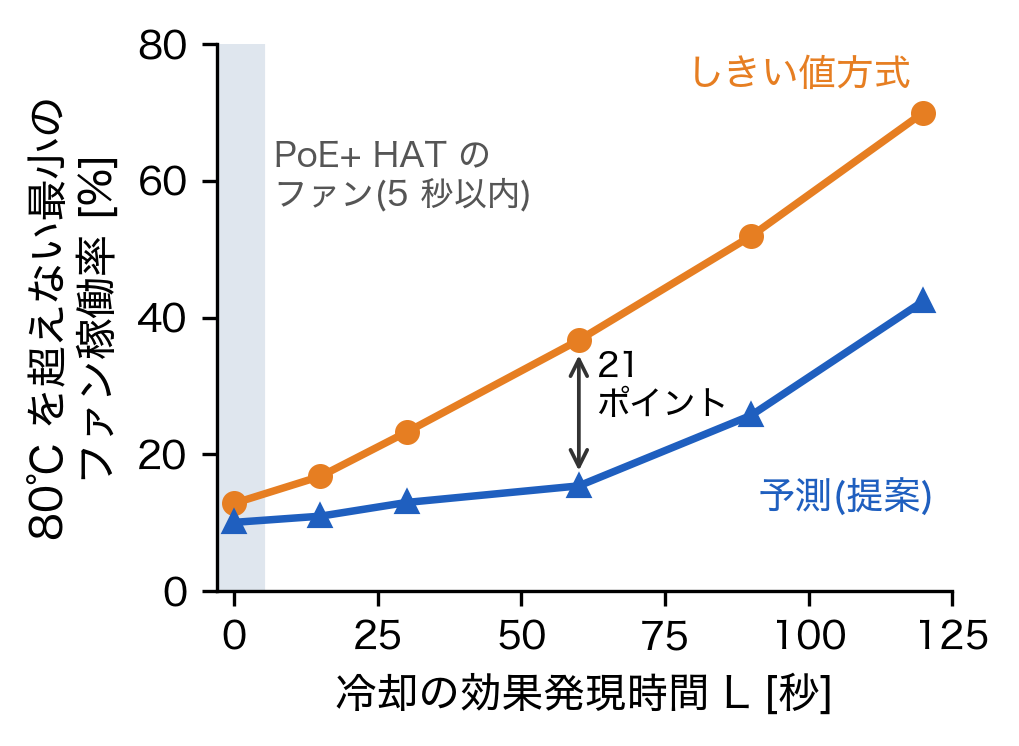
\includegraphics[width=\columnwidth]{fig_slow_cooling_resume.png}
  \caption{冷却の効果発現時間 $L$ と、80\,℃ を超えない最小のファン稼働率(シミュレーション、4 つの負荷パターンの平均。$L = 120$ 秒は、どの方式も 80\,℃ を守れない 1 本を除く)}
  \label{fig:slow}
\end{figure}

\section{考察}
\subsection{差がなかった理由}
PoE+ HAT のファンは ON にすると 5 秒以内に効き始め、冷却の効果も大きい(常時 ON で最高温度を約 19\,℃ 下げる、表\ref{tab:control})。このように速くて強い冷却では、温度が上がってから回しても間に合うため、予測の利点が小さいと考えられる。Raspi 4B でしきい値のファン制御を行った研究~\cite{benoit}でもスロットリングは防がれており、本研究の結果と合う。

\subsection{冷却が遅い場合}
部屋の空調のような効きの遅い冷却を想定し、実機で同定したモデルで冷却の効きに遅れを加えたシミュレーションを行った(条件は結果を見る前に決めた)。各方式の設定(しきい値の温度、$\alpha$)を広く変え、80\,℃ を超えない設定の中で最も少ない稼働率を比べた。ファンなどに冷却を指令してから効果が現れ始めるまでの時間を、冷却の効果発現時間 $L$ とする(制御工学でいうむだ時間)。$L$ が 15〜30 秒を超えると予測を用いる方式がしきい値方式より少ない稼働で 80\,℃ を守り(図\ref{fig:slow})、30 秒で 6〜13 ポイント、60 秒で 14〜28 ポイント少なかった。遅れの間も温度が上がるため、しきい値方式はしきい値を下げて早めに回すしかないが、予測は遅れの後の温度を見て必要なときだけ回せるためである。効きがゆっくり変わる1次遅れでは、「先読みの間ずっと OFF にしたら」という判断が悲観的すぎて差がはっきりせず、「次の周期から ON にしても間に合うか」で判断すると差が出た(後から追加した判断のため、新しい負荷で確かめた)。データセンタにもサーバのファン(速い)と空調(遅い)があり、予測は遅い冷却に用いるべきであることを示唆する。

\section{おわりに}
予測に基づくファン制御は 80\,℃ を超えずに常時 ON よりファンの稼働を約 6 割減らしたが、速くて強いファンではしきい値方式と差がなかった。予測が要るのは、効きの遅い冷却と、排熱がこもる配置であると考えられる。今後、囲った筐体で空間熱干渉が生じたときの外部熱影響の推定の効果と、効きの遅い冷却での予測の効果を実機で確かめる。

\section*{先行発表}
本研究の空間熱干渉を考慮した状態推定とマージンの手法は、情報処理学会 システムソフトウェアとオペレーティング・システム研究会で発表した~\cite{ipsj}。

\footnotesize{
\begin{thebibliography}{99}
  \setlength{\itemsep}{0pt}
  \bibitem{dayarathna} M. Dayarathna, Y. Wen, R. Fan, ``Data Center Energy Consumption Modeling: A Survey,'' IEEE Commun. Surveys \& Tutorials, Vol.18, No.1, pp.732--794, 2016.
  \bibitem{moore} J. Moore, J. Chase, P. Ranganathan, R. Sharma, ``Making Scheduling ``Cool'': Temperature-Aware Workload Placement in Data Centers,'' USENIX ATC, pp.61--74, 2005.
  \bibitem{tang} Q. Tang, S. K. S. Gupta, G. Varsamopoulos, ``Energy-Efficient Thermal-Aware Task Scheduling for Homogeneous HPC Data Centers,'' IEEE TPDS, Vol.19, No.11, pp.1458--1472, 2008.
  \bibitem{iridis} S. J. Cox, J. T. Cox, R. P. Boardman, S. J. Johnston, M. Scott, ``Iridis-pi: a low-cost, compact demonstration cluster,'' Cluster Computing, pp.349--358, 2014.
  \bibitem{kim} S. J. Kim, A. Claassen, ``How to Evaluate Fan Life,'' Electronics Cooling, 1996.
  \bibitem{ipsj} 鈴木 黎映, 知念 賢一, ``空間熱干渉を考慮した状態推定に基づく動的熱マージン制御手法,'' 情報処理学会研究報告, Vol.2026-OS-171, No.3, 2026.
  \bibitem{zanini} F. Zanini, D. Atienza, L. Benini, G. De Micheli, ``Multicore Thermal Management with Model Predictive Control,'' Proc. ECCTD, pp.711--714, 2009.
  \bibitem{sakamoto} 坂本 竜, 高橋 竜一, 深澤 良彰, ``仮想マシンの CPU 使用率の負荷予測に対する安定度を用いた動的マージン設定手法,'' 信学技報, Vol.117, No.465, pp.49--54, 2018.
  \bibitem{coskun} A. K. Coskun, T. S. Rosing, K. C. Gross, ``Proactive Temperature Management in MPSoCs,'' Proc. ISLPED, 2008.
  \bibitem{yeo} I. Yeo, C. C. Liu, E. J. Kim, ``Predictive Dynamic Thermal Management for Multicore Systems,'' Proc. DAC, pp.734--739, 2008.
  \bibitem{ogura} M. Ogura, J. Wan, S. Kasahara, ``Model Predictive Control for Energy-Efficient Operation of Data Centers with Cold Aisle Containments,'' IFAC-PapersOnLine, 2018.
  \bibitem{sasakura} 笹倉 康佑, 小松 正佳, 青木 健, 渡邊 剛, ``機械学習モデルを活用したサーバルームにおける温度環境の管理手法に関する研究(第1報),'' 空気調和・衛生工学会論文集, No.278, pp.1--8, 2020.
  \bibitem{benoit} T. Benoit-Cattin, D. Velasco-Montero, J. Fern\'{a}ndez-Berni, ``Impact of Thermal Throttling on Long-Term Visual Inference in a CPU-based Edge Device,'' arXiv:2010.06291, 2020.
\end{thebibliography}
}
\end{document}
